\section{Hyperparameter mit Bayesian Search}

% https://medium.com/data-science/a-conceptual-explanation-of-bayesian-model-based-hyperparameter-optimization-for-machine-learning-b8172278050f
% https://wandb.ai/wandb_fc/articles/reports/What-Is-Bayesian-Hyperparameter-Optimization-With-Tutorial---Vmlldzo1NDQyNzcw

% \begin{frame}{2D Vergleich Random, Grid, Bayesian}
%     % Rosenbrock funktion minimum finden
%     2d funktion minima suche mit x suchwerten. auf grafik vergleichen.
% \end{frame}

%___________________________________________________________________

% \begin{frame}[allowframebreaks]{Hyperparameter finden mit bayesian search}

% Vorschlagen neuer Punkte ein Trade-off zwischen bereits bekannten guten Punkten (exploitation) und neuen hoffentlich noch besseren Punkten (exploration) finden

% \begin{equation}
%     validation accuracy = f (parameter_1, parameter_2, ...)
%     vmax validation accuracy ?
% \end{equation}

% \begin{enumerate}
%     \item Anname für die Funktion aufstellen.
%     \item Accuracy mit neuen Parametern berechnen.
%     \item Modell der Funktion anhand des Ergebnisses anpassen.
%     \item Vermutung anstellen: Mit welchen Nächsten Werten wird der neue Beste Wert erreicht?
%     \item Zurück zu Punkt 2
% \end{enumerate}

% Bessere Ergebnisse in weniger Schritten als Random oder Grid Search

% %  P (acc | parameter) = P (paramter |score) * P(score) / P (paramter)
    
% \end{frame}

%___________________________________________________________________

\begin{frame}{Visualisierung}
    Hier GIF einfügen.
\end{frame}

%___________________________________________________________________

\begin{frame}[fragile]{Anwendung auf unser Modell}
Wie wurde es auf unserer model angewendet?
\end{frame}


%___________________________________________________________________

\begin{frame}{Bayesian Search Ergebnisse}
    \begin{figure}
        \centering
        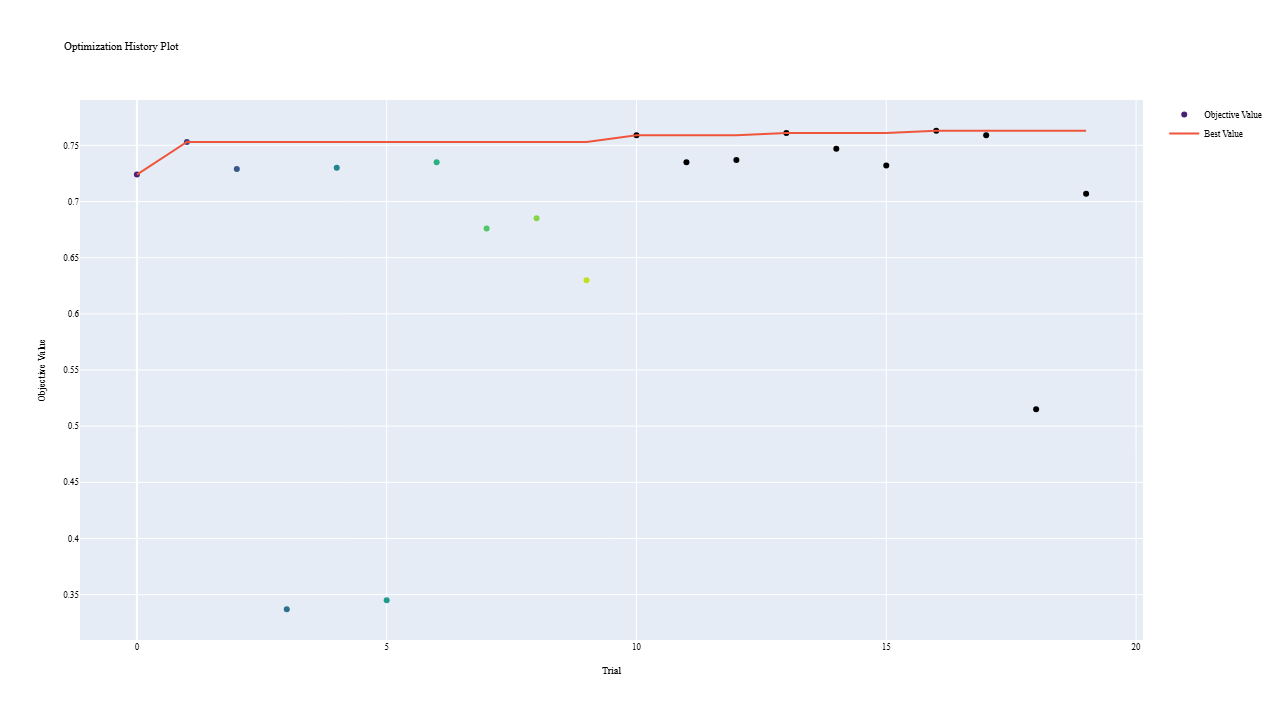
\includegraphics[width=\imagewidth, height=\imageheight, keepaspectratio]{optimization_history.png}
    \end{figure}
\end{frame}

%___________________________________________________________________

\begin{frame}{Parameter des Bayesian Search}
    \begin{figure}
        \centering
        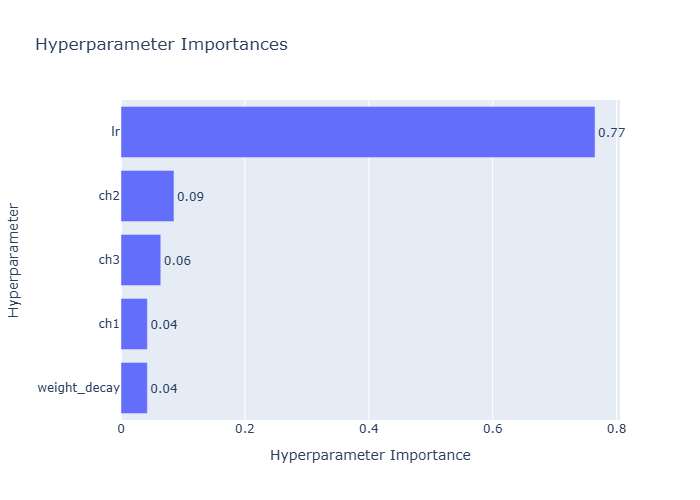
\includegraphics[width=\imagewidth, height=\imageheight, keepaspectratio]{param_importances.png}
    \end{figure}
\end{frame}